\documentclass[a4paper,11pt]{report}

\usepackage[polish]{babel}
\usepackage{blindtext}
\usepackage[T1]{fontenc}
\usepackage{booktabs}
\usepackage{graphicx}
\usepackage{wrapfig}
\usepackage{multirow}
\usepackage[export]{adjustbox}
\usepackage[nottoc,notlot,notlof]{tocbibind}

\begin{document}
\let\cleardoublepage\clearpage
\begin{figure}[ht]
\centering

\includegraphics{pjatk.png}
\end{figure}
\begin{center}
\textbf{\huge Karta Projektu}\\
\vspace{1cm}
\begin{tabular}{|p{15cm}|}
\hline
\textbf{Temat projektu:}\\Gamitude - Manage your Energy, not your Time\\ 
\hline
\textbf{Akronim:}\\GTM\\
\hline
\textbf{Opiekun:}\\Tadeusz Puźniakowski \\
\hline
\textbf{Konsultanci:}Tadeusz Puźniakowski, Marek Bednarczyk \\
\hline
\textbf{Cele projektu:}\\Dostarczenie użytkownikom narzędzia do zarządzania ich energią, opartego o najnowsze odkrycia dotyczące ludzkiej produktywności. Jednocześnie chcemy aby użytkownicy zaczęli postrzegać prace bądź naukę bardziej pozytywnie dzięki powiązaniom pracy z elementami gier RPG.\\
\hline
\textbf{Rezultaty projektu:}\\Kompletny system do zarządzania projektami opierający się na najnowszych badaniach dotyczących ludzkiej produktywności. \\
\hline
\textbf{Miary sukcesu:}\\Działający system projektów, rankingowy, workflow , web \\
\hline
\textbf{Ograniczenia:}\\Czasowe, umiejętnościowe, budżetowe \\
\hline
\end{tabular}\\
\vspace{1cm}
\begin{tabular}{|l|l|l|l|}
\hline
\textbf{Wykonawca} & \textbf{Numer albumu}& \textbf{Specjalizacja}& \textbf{Tryb studiów} \\
\hline
Robert Deyk &s17707&SI&Stacjonarne \\
\hline
Paweł Benkowski&s16569s&SI&Stacjonarne\\
\hline
Stanisław Lutkiewicz&s17535&SI&Stacjonarne \\
\hline
\end{tabular}\\
\vspace{1cm}
\begin{tabular}{|l|l|l|l|}
\hline
\textbf{Data ukończenia projektu:} & to be determend & \textbf{Recenzent:} & to be determend\\
\hline
\end{tabular}
\end{center}
\tableofcontents

\chapter{Wprowadzenie}
\section{Streszczenie}
Według pracy harwardzkiej, ludzie organizujący sobie czas pracy, patrzą tylko na czas potrzebny do wykonania jej, ignorując holistyczną naturę działania ludzkiego organizmu i potrzebę harmonijnej współpracy obu półkul mózgowych W pracy wspominane to jest jako, że czas jest surowcem skończonym jak węgiel, a energia nie jak wiatr, dlatego musimy zwracać również uwagę na energie. Dzielą się one na 4 główne: duszy, ciała, emocji i umysłu\cite{Harward}. Są różne metodologie próbujące polepszyć korzystanie z nich poprawnie, jak technika Pomodoro\cite{Pomodoro} czy technika 90/30\cite{90/30}. Pierwsza technika pozwala nam skupić się na krótsze lecz częstsze interwały czasowe po których zawsze otrzymujemy przerwę by odpocząć chwilę i przygotować się na kolejną serię. Przydatne jest to kiedy nasze zadanie możemy podzielić na mniejsze. Druga technika pozwala nam skupić się na dłuższy okres czasu, po czym otrzymujemy odpowiednio dłuższą przerwę. Dzięki tym metodą wydłużamy czas swojej efektywności przy zadaniach. Nasz system pomagający w ten sposób wykonywać zadania posiada również elementy grywalizacji\cite{grywalizacja} w postaci statystyk, które ulepszamy wykonując zadania rozwijające określone aspekty naszego życia oraz w postaci rang\cite{rangi}, które przyznawane są za osiągnięcie konkretnych statystyk. Kolejną funkcjonalnością naszego rozwiązania byłby tzw. Bullet Journal, który miałby za zadanie wizualizować rozplanowane przez użytkownika zadania na tablicy. Pokazywałaby ona jakie zadania powinien wykonać użytkownik danego dnia, tygodnia bądź miesiąca by nie przekroczyć terminu ich wykonania w podobny sposób jak Trelo\cite{trelo}. 

\section {Słownik pojęć}
	\emph{Bullet Journal – dziennik, w którym można rozplanowywać zadania}\\
	\emph{Elastic Habits – stopniowanie zadania na 3 poziomy}\\
	\emph{Projekt – Czynność bądź umiejętność, nad którą użytkownik chce pracować, nie ma podziału na podzadania, skupiający się na czasie}

\chapter {Omówienie problemu}
\section {Przedstawienie problemu}
Wielu z nas ma problem z utrzymywaniem produktywności przez dłuższy okres czasu. Bez odpowiedniego narzędzia śledzącego nawyki naszej pracy, jest to praktycznie niemożliwe. Inne dostępne rozwiązania tego typu pomijają wiele aspektów natury naszej pracy.

\section {Konkurencyjne rozwiązania}
W tej sekcji opisane zostaną konkurencyjne rozwiązania mogące konkurować z naszym. Wypisane zostaną ich negatywne, jak i pozytywne aspekty, dzięki którym jesteśmy w stanie pokazać, jak nasza aplikacja wykorzystuje te dobre cachy a odrzuca złe.
\section {Propozycja rozwiązania}
Opis ogólny działania naszej aplikacji pozwalający na zrozumieniu podstawowych działań na jakie nasz system będzie pozwalał.
\section {Kontekst systemu}
Aplikacja webowa kompatybilna z większością przeglądarek i komputerów z dostępem do Internetu. Można z niej korzystać o dowolnej porze dnia używając urządzeń mobilnych. Chcemy podzielić projekt na micro serwisy, pozwoli nam to na łatwą skalowalność i późniejsze pielęgnowanie projektu. Nasz system będzie się składał z wielu funkcjonalności, z których użytkownik będzie mógł zarządzać swoją pracą tj. zarządzanie projektami, Bullet Journal czy Elastic Habits\cite{elastic} wspierane przez system rang, system energii czy system osiągnięć. System zarządzającymi projektami pomaga nam dzielić sobie nasze zadania na sesję o określonym wymiarze czasowym wybranym przez użytkownika. Okresy te są bazowane na technikach tj. Pomodoro 25/5\cite{Pomodoro}, 90/30\cite{90/30}, flow state\cite{flow} czy Just 5\cite{just5}. Wykonywanie projektów jest gratyfikowane statystykami, które zwiększają się w zależności jakiego typu był projekt. Po spełnieniu danego warunku, użytkownik może zostać nagrodzony osiągnięciem za przekroczenie pewnego kamienia milowego w swojej pracy nad projektem. Zadaniem Bullet Journal’a jest rozplanowanie pomniejszych zadań z projektu w czasie i wizualizacja ich na tablicy, by użytkownik mógł śledzić jakie zadania musi wykonać danego dnia by wyrobić się w terminie. Elastic Habits miałby za zadanie pomóc użytkownikowi wyrobić sobie nawyk, poprzez poziomowanie sobie zaplanowanego zadania. W zależności od ogólnego samopoczucia użytkownika, może on wybrać łatwiejszą bądź trudniejszą wersję zadania, dalej utrzymując nawyk wykonywania go. \\
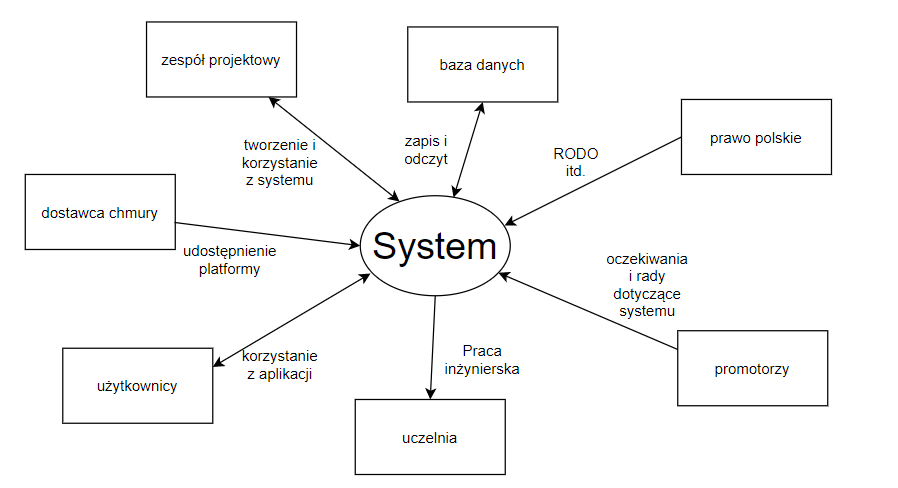
\includegraphics[width=15 cm, left]{system.png}
\section {Cele i odbiorcy systemu}
\subsection {Cele systemu}
Chcemy stworzyć nowe narzędzie do organizacji pracy z oryginalnym podejściem zaczerpniętym z systemów RPG, opartym na odkryciach w dziedzinie zarządzania energią\cite{Harward}. Chcemy aby użytkownicy korzystający z naszego narzędzia nie zarządzali wyłącznie swoim czasem, ale także i energią, która jest równie ważna. Efektem końcowym będzie aplikacja internetowa. W przyszłości planujemy rozszerzyć system o aplikację mobilną oraz desktopową. Spodziewaną korzyścią będzie wzrost produktywności długoterminowej pośród użytkowników. Produktywność użytkowników moglibyśmy sprawdzać poprzez ankiety, porównujące czas poświęcony na zadania bez korzystania z systemu oraz z nim np. użytkownik skończył zaplanowane zadanie tydzień szybciej lub pracował przez 2 godziny dłużej niż bez korzystania z systemu.\\
\subsection {Udziałowcy}
\begin{tabular}{|p{3cm}|p{11cm}|}
	\hline
	\multicolumn{2}{|l|}{\textbf{Karta Udziałowca}}\\
	\hline
	Indentyfikator&UOB01\\
	\hline
	Nazwa&Zespół projektowy\\
	\hline
	Opis&Zespół projektowy tworzy oraz opiekuje się systemem\\
	\hline
	Typ udziałowca&Ożywiony, bezpośredni\\
	\hline
	Punkt widzenia&Perspektywa twórców systemu\\
	\hline
	Ograniczenia&Brak\\
	\hline
	Wymagania&\\
	\hline
	\end{tabular}\\
	\begin{tabular}{|p{3cm}|p{11cm}|}
	\hline
	\multicolumn{2}{|l|}{\textbf{Karta Udziałowca}}\\
	\hline
	Indentyfikator&UOB02\\
	\hline
	Nazwa&Użytkownik końcowy\\
	\hline
	Opis&Przeciętny, finalny użytkownik korzystający z aplikacji\\
	\hline
	Typ udziałowca&Ożywiony, bezpośredni\\
	\hline
	Punkt widzenia&Perspektywa użytkownika\\
	\hline
	Ograniczenia&Nie ma dostępu do warstwy technicznej - bazy danych, kodu itp.\\
	\hline
	Wymagania&\\
	\hline
	\end{tabular}\\
	\begin{tabular}{|p{3cm}|p{11cm}|}
	\hline
	\multicolumn{2}{|l|}{\textbf{Karta Udziałowca}}\\
	\hline
	Indentyfikator&UOB03\\
	\hline
	Nazwa&Sponsorzy\\
	\hline
	Opis&Osoba, która finansuje projekt i egzekwuje wymagania\\
	\hline
	Typ udziałowca&Ożywiony, bezpośredni\\
	\hline
	Punkt widzenia&Perspektywa ekonomiczna\\
	\hline
	Ograniczenia&Nie powinien narzucać technologii przy tworzeniu projektu\\
	\hline
	Wymagania&\\
	\hline
	\end{tabular}\\
	\begin{tabular}{|p{3cm}|p{11cm}|}
	\hline
	\multicolumn{2}{|l|}{\textbf{Karta Udziałowca}}\\
	\hline
	Indentyfikator&UOB04\\
	\hline
	Nazwa&Wydawca\\
	\hline
	Opis&Osoba, która jest odpowiedzialna za sfinalizowanie projektu i wypuszczenie go na rynek\\
	\hline
	Typ udziałowca&Ożywiony, bezpośredni\\
	\hline
	Punkt widzenia&Perspektywa ekonomiczna\\
	\hline
	Ograniczenia&Nie powinien narzucać technologii przy tworzeniu projektu\\
	\hline
	Wymagania&\\
	\hline
	\end{tabular}\\
	\begin{tabular}{|p{3cm}|p{11cm}|}
	\hline
	\multicolumn{2}{|l|}{\textbf{Karta Udziałowca}}\\
	\hline
	Indentyfikator&UOB05\\
	\hline
	Nazwa&Promotorzy\\
	\hline
	Opis&Doradcy w sprawach dotyczących projektu\\
	\hline
	Typ udziałowca&Ożywiony, bezpośredni\\
	\hline
	Punkt widzenia&Perspektywa twórców projektu\\
	\hline
	Ograniczenia&Nie zawsze dostępni\\
	\hline
	Wymagania&\\
	\hline
	\end{tabular}\\
	\begin{tabular}{|p{3cm}|p{11cm}|}
	\hline
	\multicolumn{2}{|l|}{\textbf{Karta Udziałowca}}\\
	\hline
	Indentyfikator&UNB01\\
	\hline
	Nazwa&Media\\
	\hline
	Opis&Strony internetowe, reklamy, artykuły, audycje itp.\\
	\hline
	Typ udziałowca&Nieożywiony, bezpośredni\\
	\hline
	Punkt widzenia&Perspektywa ekonomiczna\\
	\hline
	Ograniczenia&Zero wpływu na budowę projektu\\
	\hline
	Wymagania&\\
	\hline
	\end{tabular}\\
	\begin{tabular}{|p{3cm}|p{11cm}|}
	\hline
	\multicolumn{2}{|l|}{\textbf{Karta Udziałowca}}\\
	\hline
	Indentyfikator&UNB02\\
	\hline
	Nazwa&Baza danych\\
	\hline
	Opis&Jedna, wspólna baza danych na cały system\\
	\hline
	Typ udziałowca&Nieożywiony, bezpośredni\\
	\hline
	Punkt widzenia&Perspektywa techniczna\\
	\hline
	Ograniczenia&Skończona ilość pamięci do przechowywanie informacji\\
	\hline
	Wymagania&\\
	\hline
	\end{tabular}\\
	\begin{tabular}{|p{3cm}|p{11cm}|}
	\hline
	\multicolumn{2}{|l|}{\textbf{Karta Udziałowca}}\\
	\hline
	Indentyfikator&UNB03\\
	\hline
	Nazwa&Prawo polskie\\
	\hline
	Opis&Zgodnie z RODO mamy obowiązek dbać o bezpieczeństwo danych osobowych wszyskich użytkowników\\
	\hline
	Typ udziałowca&Nieożywiony, bezpośredni\\
	\hline
	Punkt widzenia&Perspektywa prawna\\
	\hline
	Ograniczenia&Brak\\
	\hline
	Wymagania&\\
	\hline
	\end{tabular}\\
	\begin{tabular}{|p{3cm}|p{11cm}|}
	\hline
	\multicolumn{2}{|l|}{\textbf{Karta Udziałowca}}\\
	\hline
	Indentyfikator&UNB04\\
	\hline
	Nazwa&Dostawca usług chmurowych\\
	\hline
	Opis&Serwer w chmurze odpowiedzialny za przetwarzanie wszystkich żądań pomiędzy serwisami i użytkownikami końcowymi\\
	\hline
	Typ udziałowca&Nieożywiony, bezpośredni\\
	\hline
	Punkt widzenia&Perspektywa techniczna\\
	\hline
	Ograniczenia&Ograniczenia sprzętowe, specyfikacja sprzętu (np. moc procesora serwerowego, przepustowość Internetu)\\
	\hline
	Wymagania&\\
	\hline
	\end{tabular}\\
\subsection {Grupa docelowa}
Grupa docelowa to osoby, które chcą poprawić swoją higienę pracy, chcą stać się systematyczni, uniknąć przepracowania. (ładniej opisać)
\chapter {Analiza}
\section{Metodologia Pracy}
Po dłuższym namyśle, zdecydowaliśmy, że dobrym dla nas podejściem byłoby podążanie sprintami z metodologii Scrum oraz posiadanie tablicy zadań z metodologii Kanban\cite{agile}.  Sprinty wymuszają na nas ciągłą, stałą pracę by co tydzień wypuszczać nowe wersje naszego systemu. Zapewnia to stałą motywację do pracy by nie osiągnąć punktu długotrwałej stagnacji w projekcie. Tablica zadań z metodologii Kanban pozwala nam na jasne podzielenie zadań w zespole projektowym oraz ułatwia określenie w jakim stopniu dane zadanie jest wykonane.

\section {Wymagania}
\subsection {Wymagania ogólne i dziedzinowe}
		\begin{tabular}{|p{3cm}|p{2cm}|p{2cm}|p{6cm}|}
		\hline
		\multicolumn{4}{|p{12 cm}|}{Karta Wymagania}\\
		\hline
		Indentyfikator: & W01 & Priorytet: & M - must(musi być)\\
		\hline
		Nazwa & \multicolumn{3}{|p{10 cm}|}{Zwiększenie efektywności pracy użytkowników systemu}\\
		\hline
		Opis & \multicolumn{3}{|p{10 cm}|}{Końcowy produkt systemu ma za zadanie zwiększać produktywność jego użytkowników, weryfikowane jest to na podstawie prac z Harvardu i user feedback’u w postaci ankiet. }\\
		\hline
		Udziałowiec & \multicolumn{3}{|p{10 cm}|}{Wydawca, Użytkownik końcowy}\\
		\hline
		Wymagania powiązane & \multicolumn{3}{|p{10 cm}|}{Brak}\\
		\hline
		\end{tabular}\\
		\begin{tabular}{|p{3cm}|p{2cm}|p{2cm}|p{6cm}|}
		\hline
		\multicolumn{4}{|p{12 cm}|}{Karta Wymagania}\\
		\hline
		Indentyfikator: & W01 & Priorytet: & M - must(musi być)\\
		\hline
		Nazwa & \multicolumn{3}{|p{10 cm}|}{System skórek}\\
		\hline
		Opis & \multicolumn{3}{|p{10 cm}|}{Produkt będzie zarabiał na sprzedaży skórek(alternatywna oprawa graficzna i personalizacja systemu pracy)}\\
		\hline
		Udziałowiec & \multicolumn{3}{|p{10 cm}|}{Wydawca, Sponsorzy}\\
		\hline
		Wymagania powiązane & \multicolumn{3}{|p{10 cm}|}{Brak}\\
		\hline
		\end{tabular}\\
	\subsection {Wymagania funkcjonalne}
	\begin{itemize}
		\item Nazwa funkcji/usługi\\
		\begin{tabular}{|p{3cm}|p{2cm}|p{2cm}|p{6cm}|}
		\hline
		\multicolumn{4}{|p{12 cm}|}{Karta Wymagania}\\
		\hline
		Indentyfikator: & F01 & Priorytet: & M - must(musi być)\\
		\hline
		Nazwa & \multicolumn{3}{|p{10 cm}|}{System Autoryzacji użytkownika}\\
		\hline
		Opis & \multicolumn{3}{|p{10 cm}|}{Jako użytkownik muszę mieć możliwość zarejestrowania się w serwisie i późniejszego logowania się}\\
		\hline
		Kryteria akceptacji & \multicolumn{3}{|p{10 cm}|}{Bezpieczny system autoryzacji zabezpieczony przed atakami na baze danych, potwierdzenie maila po rejestracji,  jedno konta na 1 mail}\\
		\hline
		Dane wejściowe & \multicolumn{3}{|p{10 cm}|}{Brak}\\
		\hline
		Warunki początkowe & \multicolumn{3}{|p{10 cm}|}{Brak}\\
		\hline
		Warunki końcowe & \multicolumn{3}{|p{10 cm}|}{Brak}\\
		\hline
		Sytuacje wyjątkowe & \multicolumn{3}{|p{10 cm}|}{Brak}\\
		\hline
		Szczegóły implementacji & \multicolumn{3}{|p{10 cm}|}{Brak}\\
		\hline
		Udziałowiec & \multicolumn{3}{|p{10 cm}|}{Użytkownik końcowy, Zespół projektowy}\\
		\hline
		Wymagania powiązane & \multicolumn{3}{|p{10 cm}|}{Brak}\\
		\hline
		\end{tabular}\\
		\begin{tabular}{|p{3cm}|p{2cm}|p{2cm}|p{6cm}|}
		\hline
		\multicolumn{4}{|p{12 cm}|}{Karta Wymagania}\\
		\hline
		Indentyfikator: & F02 & Priorytet: & M - must(musi być)\\
		\hline
		Nazwa & \multicolumn{3}{|p{10 cm}|}{System rang użytkowników}\\
		\hline
		Opis & \multicolumn{3}{|p{10 cm}|}{Jako użytkownik podczas progresowania w trakcie używania aplikacji chciałbym być przypisywany do różnych rang}\\
		\hline
		Kryteria akceptacji & \multicolumn{3}{|p{10 cm}|}{Przypisywanie rangi do danego użytkownika oraz obliczanie jego statystyk na podstawie wykonywanych projektów}\\
		\hline
		Dane wejściowe & \multicolumn{3}{|p{10 cm}|}{Brak}\\
		\hline
		Warunki początkowe & \multicolumn{3}{|p{10 cm}|}{Brak}\\
		\hline
		Warunki końcowe & \multicolumn{3}{|p{10 cm}|}{Brak}\\
		\hline
		Sytuacje wyjątkowe & \multicolumn{3}{|p{10 cm}|}{Brak}\\
		\hline
		Szczegóły implementacji & \multicolumn{3}{|p{10 cm}|}{Brak}\\
		\hline
		Udziałowiec & \multicolumn{3}{|p{10 cm}|}{Użytkownik końcowy, Zespół projektowy}\\
		\hline
		Wymagania powiązane & \multicolumn{3}{|p{10 cm}|}{Brak}\\
		\hline
		\end{tabular}\\
		\begin{tabular}{|p{3cm}|p{2cm}|p{2cm}|p{6cm}|}
		\hline
		\multicolumn{4}{|p{12 cm}|}{Karta Wymagania}\\
		\hline
		Indentyfikator: & F03 & Priorytet: & M - must(musi być)\\
		\hline
		Nazwa & \multicolumn{3}{|p{10 cm}|}{System zarządzania energią  użytkownika}\\
		\hline
		Opis & \multicolumn{3}{|p{10 cm}|}{Jako użytkownik chcę żeby aplikacja śledziła moje zasoby energetyczne i podpowiadała jak mogę nimi lepiej zarządzać}\\
		\hline
		Kryteria akceptacji & \multicolumn{3}{|p{10 cm}|}{Zmiana zasobów energii użytkownika przy wykonywaniu konkretnych projektów lub przerw}\\
		\hline
		Dane wejściowe & \multicolumn{3}{|p{10 cm}|}{Brak}\\
		\hline
		Warunki początkowe & \multicolumn{3}{|p{10 cm}|}{Brak}\\
		\hline
		Warunki końcowe & \multicolumn{3}{|p{10 cm}|}{Brak}\\
		\hline
		Sytuacje wyjątkowe & \multicolumn{3}{|p{10 cm}|}{Brak}\\
		\hline
		Szczegóły implementacji & \multicolumn{3}{|p{10 cm}|}{Brak}\\
		\hline
		Udziałowiec & \multicolumn{3}{|p{10 cm}|}{Użytkownik końcowy, Zespół projektowy}\\
		\hline
		Wymagania powiązane & \multicolumn{3}{|p{10 cm}|}{Brak}\\
		\hline
		\end{tabular}\\
		\begin{tabular}{|p{3cm}|p{2cm}|p{2cm}|p{6cm}|}
		\hline
		\multicolumn{4}{|p{12 cm}|}{Karta Wymagania}\\
		\hline
		Indentyfikator: & F04 & Priorytet: & M - must(musi być)\\
		\hline
		Nazwa & \multicolumn{3}{|p{10 cm}|}{System zarządzania projektami użytkowników}\\
		\hline
		Opis & \multicolumn{3}{|p{10 cm}|}{Jako użytkownik chciałbym mieć możliwość dodawania, usuwania i śledzenia projektów lub zadań}\\
		\hline
		Kryteria akceptacji & \multicolumn{3}{|p{10 cm}|}{Użytkownik ma możliwość dodawania, usuwania i śledzenia projektów przez siebie stworzonych}\\
		\hline
		Dane wejściowe & \multicolumn{3}{|p{10 cm}|}{Brak}\\
		\hline
		Warunki początkowe & \multicolumn{3}{|p{10 cm}|}{Brak}\\
		\hline
		Warunki końcowe & \multicolumn{3}{|p{10 cm}|}{Brak}\\
		\hline
		Sytuacje wyjątkowe & \multicolumn{3}{|p{10 cm}|}{Brak}\\
		\hline
		Szczegóły implementacji & \multicolumn{3}{|p{10 cm}|}{Brak}\\
		\hline
		Udziałowiec & \multicolumn{3}{|p{10 cm}|}{Użytkownik końcowy, Zespół projektowy}\\
		\hline
		Wymagania powiązane & \multicolumn{3}{|p{10 cm}|}{Brak}\\
		\hline
		\end{tabular}\\
		\begin{tabular}{|p{3cm}|p{2cm}|p{2cm}|p{6cm}|}
		\hline
		\multicolumn{4}{|p{12 cm}|}{Karta Wymagania}\\
		\hline
		Indentyfikator: & F05 & Priorytet: & M - must(musi być)\\
		\hline
		Nazwa & \multicolumn{3}{|p{10 cm}|}{Bullet Journal}\\
		\hline
		Opis & \multicolumn{3}{|p{10 cm}|}{Jako użytkownik chcę mieć możliwość rozplanowania zadań na dni oraz zobaczenia ich rozłożonych w czasie na tablicy lub w postaci kalendarza}\\
		\hline
		Kryteria akceptacji & \multicolumn{3}{|p{10 cm}|}{Użytkownik może dodawać swoje zadania wraz z datami ich wykonania, które zostają zwizualizowane w postaci tablicy lub kalendarza}\\
		\hline
		Dane wejściowe & \multicolumn{3}{|p{10 cm}|}{Brak}\\
		\hline
		Warunki początkowe & \multicolumn{3}{|p{10 cm}|}{Brak}\\
		\hline
		Warunki końcowe & \multicolumn{3}{|p{10 cm}|}{Brak}\\
		\hline
		Sytuacje wyjątkowe & \multicolumn{3}{|p{10 cm}|}{Brak}\\
		\hline
		Szczegóły implementacji & \multicolumn{3}{|p{10 cm}|}{Brak}\\
		\hline
		Udziałowiec & \multicolumn{3}{|p{10 cm}|}{Użytkownik końcowy, Zespół projektowy}\\
		\hline
		Wymagania powiązane & \multicolumn{3}{|p{10 cm}|}{Brak}\\
		\hline
		\end{tabular}\\
		\begin{tabular}{|p{3cm}|p{2cm}|p{2cm}|p{6cm}|}
		\hline
		\multicolumn{4}{|p{12 cm}|}{Karta Wymagania}\\
		\hline
		Indentyfikator: & F06 & Priorytet: & C – could \\
		\hline
		Nazwa & \multicolumn{3}{|p{10 cm}|}{System osiągnięć użytkownika}\\
		\hline
		Opis & \multicolumn{3}{|p{10 cm}|}{Jako użytkownik chciałbym co jakiś czas być nagradzany za osiągnięcia przy dochodzeniu do kamieni milowych podczas korzystania z aplikacji}\\
		\hline
		Kryteria akceptacji & \multicolumn{3}{|p{10 cm}|}{Użytkownik otrzymuje osiągnięcia za przekroczenie pewnych kamieni milowych}\\
		\hline
		Dane wejściowe & \multicolumn{3}{|p{10 cm}|}{Brak}\\
		\hline
		Warunki początkowe & \multicolumn{3}{|p{10 cm}|}{Brak}\\
		\hline
		Warunki końcowe & \multicolumn{3}{|p{10 cm}|}{Brak}\\
		\hline
		Sytuacje wyjątkowe & \multicolumn{3}{|p{10 cm}|}{Brak}\\
		\hline
		Szczegóły implementacji & \multicolumn{3}{|p{10 cm}|}{Brak}\\
		\hline
		Udziałowiec & \multicolumn{3}{|p{10 cm}|}{Użytkownik końcowy, Zespół projektowy}\\
		\hline
		Wymagania powiązane & \multicolumn{3}{|p{10 cm}|}{Brak}\\
		\hline
		\end{tabular}\\
		\begin{tabular}{|p{3cm}|p{2cm}|p{2cm}|p{6cm}|}
		\hline
		\multicolumn{4}{|p{12 cm}|}{Karta Wymagania}\\
		\hline
		Indentyfikator: & F07 & Priorytet: & C – could\\
		\hline
		Nazwa & \multicolumn{3}{|p{10 cm}|}{System rankingowy użytkowników}\\
		\hline
		Opis & \multicolumn{3}{|p{10 cm}|}{Jako użytkownik chciałbym mieć dostęp do tablic rankingowych gdzie mógłbym porównywać swoje osiągniecia z innymi użytkownikami }\\
		\hline
		Kryteria akceptacji & \multicolumn{3}{|p{10 cm}|}{Użytkownik jest w stanie sprawdzić swoją pozycję w rankingu dotyczącą danego projektu}\\
		\hline
		Dane wejściowe & \multicolumn{3}{|p{10 cm}|}{Brak}\\
		\hline
		Warunki początkowe & \multicolumn{3}{|p{10 cm}|}{Brak}\\
		\hline
		Warunki końcowe & \multicolumn{3}{|p{10 cm}|}{Brak}\\
		\hline
		Sytuacje wyjątkowe & \multicolumn{3}{|p{10 cm}|}{Brak}\\
		\hline
		Szczegóły implementacji & \multicolumn{3}{|p{10 cm}|}{Brak}\\
		\hline
		Udziałowiec & \multicolumn{3}{|p{10 cm}|}{Użytkownik końcowy, Zespół projektowy}\\
		\hline
		Wymagania powiązane & \multicolumn{3}{|p{10 cm}|}{Brak}\\
		\hline
		\end{tabular}\\
		\begin{tabular}{|p{3cm}|p{2cm}|p{2cm}|p{6cm}|}
		\hline
		\multicolumn{4}{|p{12 cm}|}{Karta Wymagania}\\
		\hline
		Indentyfikator: & F08 & Priorytet: & C – could \\
		\hline
		Nazwa & \multicolumn{3}{|p{10 cm}|}{System znajomych użytkowników}\\
		\hline
		Opis & \multicolumn{3}{|p{10 cm}|}{Jako użytkownik chciałbym móc dodawać innych użytkowników do swojej listy znajomych żeby sprawdzać ich postępy}\\
		\hline
		Kryteria akceptacji & \multicolumn{3}{|p{10 cm}|}{Użytkownik może dodawaj znajomych, wyświetlanych w formie listy, u których może sprawdzać ich postępy}\\
		\hline
		Dane wejściowe & \multicolumn{3}{|p{10 cm}|}{Brak}\\
		\hline
		Warunki początkowe & \multicolumn{3}{|p{10 cm}|}{Brak}\\
		\hline
		Warunki końcowe & \multicolumn{3}{|p{10 cm}|}{Brak}\\
		\hline
		Sytuacje wyjątkowe & \multicolumn{3}{|p{10 cm}|}{Brak}\\
		\hline
		Szczegóły implementacji & \multicolumn{3}{|p{10 cm}|}{Brak}\\
		\hline
		Udziałowiec & \multicolumn{3}{|p{10 cm}|}{Użytkownik końcowy, Zespół projektowy}\\
		\hline
		Wymagania powiązane & \multicolumn{3}{|p{10 cm}|}{Brak}\\
		\hline
		\end{tabular}\\
		\begin{tabular}{|p{3cm}|p{2cm}|p{2cm}|p{6cm}|}
		\hline
		\multicolumn{4}{|p{12 cm}|}{Karta Wymagania}\\
		\hline
		Indentyfikator: & F09 & Priorytet: & C – could\\
		\hline
		Nazwa & \multicolumn{3}{|p{10 cm}|}{Energy Assistant}\\
		\hline
		Opis & \multicolumn{3}{|p{10 cm}|}{Jako użytkownik chciałbym żeby moje rzeczywiste poziomy energii były lepiej rozpoznawane }\\
		\hline
		Kryteria akceptacji & \multicolumn{3}{|p{10 cm}|}{Użytkownik zależnie jaki prowadzi tryb życia, bądź w zależności od jego warunków fizycznych jak i psychicznych miałby dostosowywaną ilość energii na dany dzień}\\
		\hline
		Dane wejściowe & \multicolumn{3}{|p{10 cm}|}{Brak}\\
		\hline
		Warunki początkowe & \multicolumn{3}{|p{10 cm}|}{Brak}\\
		\hline
		Warunki końcowe & \multicolumn{3}{|p{10 cm}|}{Brak}\\
		\hline
		Sytuacje wyjątkowe & \multicolumn{3}{|p{10 cm}|}{Brak}\\
		\hline
		Szczegóły implementacji & \multicolumn{3}{|p{10 cm}|}{Brak}\\
		\hline
		Udziałowiec & \multicolumn{3}{|p{10 cm}|}{Użytkownik końcowy, Zespół projektowy}\\
		\hline
		Wymagania powiązane & \multicolumn{3}{|p{10 cm}|}{Brak}\\
		\hline
		\end{tabular}\\
		\begin{tabular}{|p{3cm}|p{2cm}|p{2cm}|p{6cm}|}
		\hline
		\multicolumn{4}{|p{12 cm}|}{Karta Wymagania}\\
		\hline
		Indentyfikator: & F10 & Priorytet: & C – could\\
		\hline
		Nazwa & \multicolumn{3}{|p{10 cm}|}{Elastic Habits}\\
		\hline
		Opis & \multicolumn{3}{|p{10 cm}|}{Jako użytkownik chciałbym móc podzielić swoje zadanie na różne poziomy trudności }\\
		\hline
		Kryteria akceptacji & \multicolumn{3}{|p{10 cm}|}{Użytkownik może wybrać z dany poziom trudności zadania by wyrobić sobie nawyk wykonywania go.}\\
		\hline
		Dane wejściowe & \multicolumn{3}{|p{10 cm}|}{Brak}\\
		\hline
		Warunki początkowe & \multicolumn{3}{|p{10 cm}|}{Brak}\\
		\hline
		Warunki końcowe & \multicolumn{3}{|p{10 cm}|}{Brak}\\
		\hline
		Sytuacje wyjątkowe & \multicolumn{3}{|p{10 cm}|}{Brak}\\
		\hline
		Szczegóły implementacji & \multicolumn{3}{|p{10 cm}|}{Brak}\\
		\hline
		Udziałowiec & \multicolumn{3}{|p{10 cm}|}{Użytkownik końcowy, Zespół projektowy}\\
		\hline
		Wymagania powiązane & \multicolumn{3}{|p{10 cm}|}{Brak}\\
		\hline
		\end{tabular}\\
		\item Interfejs z otoczeniem\\
		\begin{tabular}{|p{3cm}|p{2cm}|p{2cm}|p{6cm}|}
		\hline
		\multicolumn{4}{|p{12 cm}|}{Karta Wymagania}\\
		\hline
		Indentyfikator: & I01 & Priorytet: & M – must (musi być)\\
		\hline
		Nazwa & \multicolumn{3}{|p{10 cm}|}{Integracja mikro serwisów}\\
		\hline
		Opis & \multicolumn{3}{|p{10 cm}|}{Nasz projekt strukturalnie będzie zbudowany z wielu mikro serwisów i wymagana jest integracja miedzy nimi(komunikatywność)}\\
		\hline
		Kryteria akceptacji & \multicolumn{3}{|p{10 cm}|}{Funkcje w każdym serwisie umożliwiające komunikowanie się z innymi serwisami}\\
		\hline
		Dane wejściowe & \multicolumn{3}{|p{10 cm}|}{Brak}\\
		\hline
		Warunki początkowe & \multicolumn{3}{|p{10 cm}|}{Brak}\\
		\hline
		Warunki końcowe & \multicolumn{3}{|p{10 cm}|}{Brak}\\
		\hline
		Sytuacje wyjątkowe & \multicolumn{3}{|p{10 cm}|}{Brak}\\
		\hline
		Szczegóły implementacji & \multicolumn{3}{|p{10 cm}|}{Brak}\\
		\hline
		Udziałowiec & \multicolumn{3}{|p{10 cm}|}{Zespół projektowy}\\
		\hline
		Wymagania powiązane & \multicolumn{3}{|p{10 cm}|}{Brak}\\
		\hline
		\end{tabular}\\
		\begin{tabular}{|p{3cm}|p{2cm}|p{2cm}|p{6cm}|}
		\hline
		\multicolumn{4}{|p{12 cm}|}{Karta Wymagania}\\
		\hline
		Indentyfikator: & I02 & Priorytet: & M – must (musi być)\\
		\hline
		Nazwa & \multicolumn{3}{|p{10 cm}|}{Baza danych}\\
		\hline
		Opis & \multicolumn{3}{|p{10 cm}|}{Jedna zintegrowana baza danych dla wszystkich serwisów}\\
		\hline
		Kryteria akceptacji & \multicolumn{3}{|p{10 cm}|}{Baza danych w MongoDB która będzie obsługiwać wszystkie mikro serwisy projektu, będzie posiadała dane użytkowników i wszystkiego co jest związane z aplikacja}\\
		\hline
		Dane wejściowe & \multicolumn{3}{|p{10 cm}|}{Brak}\\
		\hline
		Warunki początkowe & \multicolumn{3}{|p{10 cm}|}{Brak}\\
		\hline
		Warunki końcowe & \multicolumn{3}{|p{10 cm}|}{Brak}\\
		\hline
		Sytuacje wyjątkowe & \multicolumn{3}{|p{10 cm}|}{Brak}\\
		\hline
		Szczegóły implementacji & \multicolumn{3}{|p{10 cm}|}{Brak}\\
		\hline
		Udziałowiec & \multicolumn{3}{|p{10 cm}|}{Zespół projektowy}\\
		\hline
		Wymagania powiązane & \multicolumn{3}{|p{10 cm}|}{Brak}\\
		\hline
		\end{tabular}\\
	\end{itemize}
	\subsection {Wymagania pozafunkcjonalne}
	\begin{tabular}{|p{3cm}|p{2cm}|p{2cm}|p{6cm}|}
		\hline
		\multicolumn{4}{|p{12 cm}|}{Karta Wymagania}\\
		\hline
		Indentyfikator: & NF01 & Priorytet: & M – must (musi być)\\
		\hline
		Nazwa & \multicolumn{3}{|p{10 cm}|}{C\#}\\
		\hline
		Opis & \multicolumn{3}{|p{10 cm}|}{Serwisy backendowe powinny być napisane w C\#}\\
		\hline
		Udziałowiec & \multicolumn{3}{|p{10 cm}|}{Zespół projektowy, Wydawca}\\
		\hline
		Wymagania powiązane & \multicolumn{3}{|p{10 cm}|}{Brak}\\
		\hline
		\end{tabular}\\
		\begin{tabular}{|p{3cm}|p{2cm}|p{2cm}|p{6cm}|}
		\hline
		\multicolumn{4}{|p{12 cm}|}{Karta Wymagania}\\
		\hline
		Indentyfikator: & NF02 & Priorytet: & M – must (musi być)\\
		\hline
		Nazwa & \multicolumn{3}{|p{10 cm}|}{React.js}\\
		\hline
		Opis & \multicolumn{3}{|p{10 cm}|}{Serwis frontendowy powinien być napisany korzystając z biblioteki React.js}\\
		\hline
		Udziałowiec & \multicolumn{3}{|p{10 cm}|}{Zespół projektowy, Wydawca}\\
		\hline
		Wymagania powiązane & \multicolumn{3}{|p{10 cm}|}{Brak}\\
		\hline
		\end{tabular}\\
		\begin{tabular}{|p{3cm}|p{2cm}|p{2cm}|p{6cm}|}
		\hline
		\multicolumn{4}{|p{12 cm}|}{Karta Wymagania}\\
		\hline
		Indentyfikator: & NF03 & Priorytet: & M – must (musi być)\\
		\hline
		Nazwa & \multicolumn{3}{|p{10 cm}|}{Czas wdrożenia }\\
		\hline
		Opis & \multicolumn{3}{|p{10 cm}|}{System należy wdrożyć do końca semestru zimowego 2020/2021}\\
		\hline
		Udziałowiec & \multicolumn{3}{|p{10 cm}|}{Zespół projektowy, Promotorzy, Uczelnia, Wydawca}\\
		\hline
		Wymagania powiązane & \multicolumn{3}{|p{10 cm}|}{Brak}\\
		\hline
		\end{tabular}\\
		\begin{tabular}{|p{3cm}|p{2cm}|p{2cm}|p{6cm}|}
		\hline
		\multicolumn{4}{|p{12 cm}|}{Karta Wymagania}\\
		\hline
		Indentyfikator: & NF04 & Priorytet: & M – must (musi być)\\
		\hline
		Nazwa & \multicolumn{3}{|p{10 cm}|}{System powinien być dostępny 24 godziny na dobę, 7 dni w tygodniu}\\
		\hline
		Opis & \multicolumn{3}{|p{10 cm}|}{Dostęp do systemu powinien być umożliwiony w dowolnej chwili danego dnia}\\
		\hline
		Udziałowiec & \multicolumn{3}{|p{10 cm}|}{Zespół projektowy, Użytkownik końcowy, Wydawca}\\
		\hline
		Wymagania powiązane & \multicolumn{3}{|p{10 cm}|}{Brak}\\
		\hline
		\end{tabular}\\
	\subsection {Wymagania na środowisko docelowe}
	\begin{tabular}{|p{3cm}|p{2cm}|p{2cm}|p{6cm}|}
		\hline
		\multicolumn{4}{|p{12 cm}|}{Karta Wymagania}\\
		\hline
		Indentyfikator: & ŚD01 & Priorytet: & M – must (musi być)\\
		\hline
		Nazwa & \multicolumn{3}{|p{10 cm}|}{Kompatybilność przeglądarek}\\
		\hline
		Opis & \multicolumn{3}{|p{10 cm}|}{Produkt końcowy musi być kompatybilny z 3 najnowszymi wersjami popularnych przeglądarek}\\
		\hline
		Kryteria akceptacji & \multicolumn{3}{|p{10 cm}|}{System kompatybilny z 3 najnowszymi wersjami przeglądarek Google Chrome i Mozilla Firefox}\\
		\hline
		Udziałowiec & \multicolumn{3}{|p{10 cm}|}{Zespół projektowy, Użytkownik końcowy, Wydawca}\\
		\hline
		Wymagania powiązane & \multicolumn{3}{|p{10 cm}|}{Brak}\\
		\hline
		\end{tabular}\\
	\section {Wymagania jakościowe i inne}
	\begin{itemize}
		\item System szyfrowania danych użytkowników: szyfrowanie transmisji, haseł i ciasteczek
		\item Wsparcie dla ostatnich trzech wersji Google Chrome i Mozilla Firefox
		\item System dostępny 24 godziny na dobę z wyłączeniem prac technicznych
		\item System ma być łatwy w obsłudze – średnio 5 kliknięć na wykonanie dowolnej 
	\end{itemize}
\chapter {Projektowanie}
\section {Główne Funkcjonalności Projektu}
\subsection {Projekty}
\subsection {Bullet Journal}
\subsection {Sklep Gamitude Themes}
\subsection {Statystyki użytkowników}
\section {Wizja konstrukcyjna}
\subsection{Frontend} 
\subsection{Backend}
\subsection{Baza Danych}
\subsection{Chmura}
\section{Narzędzia}
Opisanie narzędzi wykorzystanych do tworzenia projektu (slack, azure dev, google cloud itd.)
\section{Technologie}
		\begin{itemize}
			\item React/Redux/MUI - frontend
			\item .NET - Backend
			\item MongoDB/Postgres - baza danych
		\end{itemize}

\chapter {Implementacja}

\section {Rozpoznanie dziedzinowe}
\subsection {Założenia sprintu}
Każdy członek zespołu wybrał sobie pewien sposób na zarządzanie swoimi zadaniami w ciągu dnia w celu zbadania dziedziny problemu.
\subsection {Wykonane zadania}
Paweł: Używanie metodologi Pomodoro i Ulthradian rythm do codziennych zadań. Przerabianie kursu React.
Robert: Rozplanowywanie zadań za pomocą GTD (Getting Things Done)
Stanisław: Zapoznanie się i zastosowanie Bullet Journal'a oraz szukanie alternatyw dla narzędzi do dokumentowania projektu (Enterprise Architect, Github).
\subsection {Napotkane problemy}
Brak zastępcy dla programu Enterprise Architect. Spór dotyczący wyboru Azure Repos a Github'em.

\section {Wstępna dokumentacja}
\subsection {Założenia sprintu}
Podczas sprintu, zespół miał za zadanie wytworzyć wstępne dokumenty DZW i SWS oraz znalezienie sposobu na wersjonowanie w EA.
\subsection {Wykonane zadania}
Paweł: Wytworzenie wstępnej wersji dokumentu DZW. Przerabianie kursu React.
Robert: Wytworzenie wstępnej wersji dokumentu SWS.
Stanisław: Rozpoznanie dotyczące wersjonowania w EA.
\subsection {Napotkane problemy}
Wersjonowanie w EA dostępne tylko po wykupieniu licencji.

\section {Use Case + WPP}
\subsection {Założenia sprintu}
Przygotowanie pierwszych diagramów Use Case. Wytworzenie dokumentu WPP.
\subsection {Wykonane zadania}
Paweł: Wytworzenie paru Use Case'ów w programie EA. Przerabianie kursu React.
Robert: Stworzenie dokumentu WPP oraz jednego z Use Case'ów.
Stanisław: Wytworzenie paru Use Case'ów w programie EA.
\subsection {Napotkane problemy}
Brak napotkanych problemów.

\section {Dalsza praca przy SWS}
\subsection {Założenia sprintu}
Doprecyzowanie wymagań systemowych oraz niefunkcjonalnych w dokumencie SWS. Podjąć decyzję odnośnie architektury systemu.
\subsection {Wykonane zadania}
Zespół: Wspólna praca nad SWS oraz wybranie architektury mikroserwisowej dla systemu.
Paweł: Przerabianie kursu React.
\subsection {Napotkane problemy}
Brak napotkanych problemów.

\section {Przygotowanie narzędzi do tworzenia systemu}
\subsection {Założenia sprintu}
Znalezienie i skonfigurowanie platformy do komunikacji zespołu, stworzenie repozytoriów dla każdego mikroserwisu oraz przygotowanie wstępnego mockup'u UI dla systemu.
\subsection {Wykonane zadania}
Paweł: Stworzenie pierwszego mockup'u UI dla systemu. Przerabianie kursu React. 
Stanisław: Stworzenie repozytoriów dla wszystkich mikroserwisów oraz przygotowanie platformy Slack do komunikacji zespołu.
\subsection {Napotkane problemy}
Rozmowy grupowe na platformie Slack były płatne, więc musiliśmy znaleźć alternatywę dla domyślnych rozmów.

\section {Diagramy funkcjonalności, wymagania bazy danych oraz responsywne rozłożenie strony}
\subsection {Założenia sprintu}
Każdy z członków zespołu stworzy diagram funkcjonalności dla swojego mikroserwisu, który pomoże w określeniu wymagań funkcjonalnych. Utworzony zostanie diagram wymagań dla bazy danych oraz wykres Gantt’a i wstępne ułożenie poszczególnych komponentów na stronie.
\subsection {Wykonane zadania}
Zespół: Tworzenie wykresu Gantt'a.
Paweł: Utworzenie responsywnego rozłożenia strony. 
Robert: Stworzenie diagramu funkcjonalności. 
Stanisław: Stworzenie diagramu funkcjonalności oraz bazy danych.
\subsection {Napotkane problemy}
Znalezienie darmowego narzędzia dla wykresu Gantt'a.

\section {Diagramy klas i nawigacja strony}
\subsection {Założenia sprintu}
Członkowie zespołu odpowiedzialni za backend projektu wykonają diagramy klas dla swoich serwisów, utworzą struktury plików dla poszczególnych mikroserwisów, przygotują routing dla nich. Zostanie stworzona nawigacja strony.
\subsection {Wykonane zadania}
Robert i Stanisław: Utworzenie diagramu klas dla mikroserwisów oraz struktury plików dla nich.
Paweł: Implementacja nawigacji strony. 
Stanisław: Stworzenie routingu dla mikroserwisu projektów.
\subsection {Napotkane problemy}
Robert nie przygotował routingu.

\section {Diagram sekwencji oraz statystyki i energie na stronie}
\subsection {Założenia sprintu}
Zostanie utworzony diagram sekwencji pozwalający zobrazować przepływ danych w projekcie. Utworzone zostaną widoki statystyk i energii na stronie.
\subsection {Wykonane zadania}
Robert i Stanisław: Utworzenie diagramu sekwencji.
Paweł: Implementacja widoków statystyk i energii. 
Robert: Utworzono routing w mikroserwisie rang.
Stanisław: Modyfikacja modelu projektów w bazie danych.
\subsection {Napotkane problemy}
Brak napotkanych problemów.

\section {Algorytmy oraz rangi na stronie}
\subsection {Założenia sprintu}
Stworzenie algorytmów odpowiedzialnych za przyznawanie rangi oraz za wzrost lub spadek energii. Zaimplementowanie struktury bazy danych zgodnej z dokumentacją oraz utworzenie rang na frontendzie.
\subsection {Wykonane zadania}
Paweł: Implementacja widoków rang. 
Robert: Algorytm przyznawania rang i statystyk.
Stanisław: Algorytm wzrostu i spadku energii. Implementacja struktury bazy danych.
\subsection {Napotkane problemy}
Brak napotkanych problemów.

\section {Firebase, Heroku, projekty}
\subsection {Założenia sprintu}
Utworzenie konta firebase dla projektu, schematów modeli bazy danych dla mikroserwisów, przeniesienie bazy danych na platrofmę Heroku, utworzenie wyglądu projektów na frontendzie.
\subsection {Wykonane zadania}
Robert i Stanisław: Stworzenie schematów modeli bazy danych dla mikroserwisów.
Paweł: Implementacja widoków projektów. Refaktoryzacja dotychczasowego kodu. 
Stanisław: Przeniesienie bazy danych na platrofmę Heroku. Utworzenie konta firebase dla projektu.
\subsection {Napotkane problemy}
Modele rang i workflow nie zgodne z założeniami, do poprawy w następnym sprint'ie.

\section {Firebase autoryzacja, API refactor}
\subsection {Założenia sprintu}
Dodanie rang do bazy danych, serwisu firebase do projektu, funkcji tworzenia użytkownika przez firebase, refaktoryzajca serwisów workflow i projektów, utworzenie strony logowania i rejestracji na frontendzie oraz poprawienie wyglądu projektów.
\subsection {Wykonane zadania}
Robert i Stanisław: Poprawa modeli rang i workflow.
Paweł: Utworzenie strony logowania i rejestracji na frontendzie oraz poprawienie wyglądu projektów, dodanie serwisu firebase do projektu oraz funkcji tworzenia użytkownika przez firebase.
Robert: Dodanie rang do bazy danych.
Stanisław: Refaktoryzajca serwisów workflow i projektów,
\subsection {Napotkane problemy}
Algorytmy niedostosowane do działania w czasie. Poprawa na następny tydzień.

\section {Integracja}
\subsection {Założenia sprintu}
Ukończonie prace nad algorytmami związanymi z przyznawaniem rang oraz zmianą energii, dodanie wszystkich działających endpoint’ów do serwisu frontendowego.
\subsection {Wykonane zadania}
Robert i Stanisław: Dostosowanie algorytmów do wymagań. 
Paweł: Integracja z API.
\subsection {Napotkane problemy}
Problem z integracją frontendu z API.

\section {Prezentacja i demo}
\subsection {Założenia sprintu}
Utworzenie prezentacji projektu oraz pokazowego dema działania aplikacji.
\subsection {Wykonane zadania}
Robert: Wykonanie pokazowego dema. 
Paweł: Stworzenie prezentacji.
\subsection {Napotkane problemy}
Przez problemy z integracją frontendu z API, część projektu musiała zostać postawiona na mockup'ach.

\section {Zmiana technologii na backendzie, retrospekcja}
\subsection {Założenia sprintu}
Przyjrzenie się powstałemu już systemowi i wyznaczenie kierunku dalszych prac.
\subsection {Wykonane zadania}
Zespół: Ustalenie zmiany technologi backendowej na C\#, zaakceptowanie pomysłu na utworzenie sklepu z motywami dla aplikacji, wspólna decyzja o zrezygnowaniu z firebase'a
Paweł: Utworzenie nowego formularza logowania i rejestracji bez firebase'a
Stanisław: Rozpozczęcie prac nad przerabianiem serwisów z node.js na C\#, praca nad serwisem autoryzacji użytkownika, przystosowanie chmury do pracy z technologią .NET, wyeksportowanie obecną bazę danych do pliku lokalnego w razie zmiany bazy.
\subsection {Napotkane problemy}
Brak napotkanych problemów

\section {Festiwal pomysłów i mockup'y}
\subsection {Założenia sprintu}
Szukanie nowych pomysłów na funkcjonalności. Stworzenie mockupów dla strony głównej oraz bullet journala. 
\subsection {Wykonane zadania}
Paweł: Elastic habits, Just 5, flow state, Energy asistant, system osiągnięć czy system rankingu między graczami.
Robert: Stworzenie mockup'u strony głównej oraz Bullet Journal'a.
Stanisław: Pomysł na zbieranie informacji o użytkownikach dla późniejszej sprzedaży.
\subsection {Napotkane problemy}
Brak napotkanych problemów

\section {Festiwal pomysłów ciąg dalszy}
\subsection {Założenia sprintu}
Zakonczonie prac nad serwisem projektów oraz zaczęcie prac nad serwisem rang. Dalsze szukanie pomysłów.
\subsection {Wykonane zadania}
Paweł: skills, wybieranie innego zadania jako przerwy, tworzenie statystyk użytkownika z danych zadań.
Stanisław: Zakonczono pracę nad serwisem projektów oraz zaczęto nad serwisem rang.
\subsection {Napotkane problemy}
Brak napotkanych problemów

\section {Autoryzacja i budowanie bibliografii}
\subsection {Założenia sprintu}
Połączenie frontendu z serwisem logowania i rejestracji. Zbudowanie podstawowej bibliografii.
\subsection {Wykonane zadania}
Paweł i Stanisław: Połączenie frontendu z przepisanym serwisem.
Robert: Zebranie danych dotyczących źródeł informacji do bibliografii.
\subsection {Napotkane problemy}
Brak napotkanych problemów

\section {Smartwatch'e i MBTI}
\subsection {Założenia sprintu}
Szukanie informacji na temat wykorzystania smartwatchy w aplikacji. Rozpoznanie w zakresie różnych typów użytkowników systemu. 
\subsection {Wykonane zadania}
Paweł i Robert: Wykonanie badania MBTI.
Stanisław: Pomysł na integracje aplikacji z Google Calendar.
\subsection {Napotkane problemy}
Brak napotkanych problemów

\section {Odnowienie dokumentacji i bezpieczeństwo}
\subsection {Założenia sprintu}
Zebranie całej starej dokumentacji w jedno miejsce. Zapewnienie bezpieczeństwa aplikacji.  
\subsection {Wykonane zadania}
Zespół: Modyfikacja dokumentu DZW.
Robert: Zebranie całej dokumentacji i wstawienie jej na platformę Github, napisanie streszczenia projektu.
Stanisław: Szukanie informacji na temat certyfikatu ssl.
\subsection {Napotkane problemy}
Brak napotkanych problemów

\section {Autoryzacja, dokumentacja}
\subsection {Założenia sprintu}
Poprawa bibliografii, zebranie historii sprintów, poprawa wyglądu systemu autoryzacji użytkownika po stronie frontendu.
\subsection {Wykonane zadania}
Robert: Stworzenie bibliografii zgodnie z zaleceniami dziekana, skończenie spisywanie historii sprintów do obecnego stanu, wstępne poprawki do dokumentu SWS
Paweł: Implementacja poprawek systemu autoryzacji użytkownika po stronie frontendu
Stanisław: Research na temat architektury systemu.
\subsection {Napotkane problemy}
Brak napotkanych problemów

\section {Końcowe prace nad przepisanymi serwisami}
\subsection {Założenia sprintu}
Zintegrowanie serwisu projektów, uaktualnienie dokumentów o uwagi promotora, kończenie prac nad serwisem statystyk i energii.
\subsection {Wykonane zadania}
Paweł: Integracja serwisu projektów, walidacja wprowadzonych danych na frontend
Robert: Uzupełnienie DZW o nowe funkcjonalności, stworzenie dokumentu SWS oraz ulepszenie o uwagi promotora
Stanisław: Końcowe prace nad serwisem statystyk i energii, naprawianie błędów w stworzonych serwisach.
\subsection {Napotkane problemy}
Brak napotkanych problemów

\section {Integracja i LaTeX}
\subsection {Założenia sprintu}
Integracja zakończonnych mikroserwiów, przygotowania do przepisania dokumentacji na latex.
\subsection {Wykonane zadania}
Robert: Wstępna wersja widoku Gamitude Themes, research na temat języka do tworzenia dokumentacji LaTeX
Paweł: Obsługa błędów dla projektów, integracja serwisu statystyk i energii
Stanisław: skończenie serwisu statystyk, czytanie o mikroserwisach, prace nad cronem
\subsection {Napotkane problemy}
Brak napotkanych problemów

\section {Przepisywanie dokumentacji}
\subsection {Założenia sprintu}
Stworzenie domyślengo dokumentu dla pracy oraz rozpoczęcie prac nad przepisywaniem pozostałych dokumentów.
\subsection {Wykonane zadania}
Robert: przerabianie dokumentów na latex 
Paweł: research na temat połączenia kalendarza i Bullet Journal'a  
Stanisław: przerabianie kursu o identity serwer 4 
\subsection {Napotkane problemy}
Brak napotkanych problemów




\section {Podpowiedzi i naprawa błędów}
\subsection {Założenia sprintu}
Dodanie podpowiedzi dla użytkownika by ułatwić zapoznawanie się z systemem. Naprawa błędów w przeliczaniu statystyk
\subsection {Wykonane zadania}
Robert: dodanie karty projektów w latex.
Paweł: Stworzenie podpowiedzi dla użytkowników na stronie. 
Stanisław: Poprawa błędów w obliczaniu statystyk.  
\subsection {Napotkane problemy}
Brak napotkanych problemów.

\section {DZW i integracja rang}
\subsection {Założenia sprintu}
Zintegrowanie przepisanego systemu rang, przepisanie dokumentu DZW na LaTeX.
\subsection {Wykonane zadania}
Robert: Dodanie DZW do latex dokumentu, przerobienie bibliografi. 
Paweł: Dodanie więcej podpowiedzi do strony, dodawanie projektu przeniesione do modala, połączenie API rang z frontendem.
Stanisław: Naprawiony system rang, dodanie load balancera do projektu by zoptymalizować go w Kubernetes'ie.    
\subsection {Napotkane problemy}
Brak napotkanych problemów.

\section {SWS i nowe minutniki}
\subsection {Założenia sprintu}
Wstępna implementacja nowych minutników, zastosowanie certyfikatu ssl na stronie, przepisanie SWS do LaTeX.
\subsection {Wykonane zadania}
Robert: SWS przepisany do latex .
Paweł: Implementacja minutników flow state, just 5 i custom time.  
Stanisław: Dodanie certyfikatu SSL.  
\subsection {Napotkane problemy}
Brak napotkanych problemów.

\section {Strona główna i przerwy}
\subsection {Założenia sprintu}
Wstępna implementacja przerw, stworzenie pierwszej wersji strony głownej z użyciem parallax, .
\subsection {Wykonane zadania}
Robert: Pierwsza wersja strony głównej w parallax 
Paweł: Rozpoczęcie implementacji przerw 
Stanisław: Dodanie opcji spadku dziennych statystyk  
\subsection {Napotkane problemy}
Brak napotkanych problemów.

\section {Experymenty z Azure, ulepszanie parallax'a}
\subsection {Założenia sprintu}
Stworzenie repopozytorium dla serwisu użytkownika, sprawdzenie działania bazy MS SQL na Azure.
\subsection {Wykonane zadania}
Robert: Ulepszanie strony głównej z parallax'em.
Paweł: Przygotowanie teoretyczne do dodania TypeScript'u do projektu.
Stanisław: Wstawienie bazy MS SQL na Azure, stworzenie repopozytorium dla serwisu użytkownika.  
\subsection {Napotkane problemy}
Brak napotkanych problemów.

\section {Zbieranie informacji}
\subsection {Założenia sprintu}
Poprawa strony głównej, znaleźć informacje dotyczące mikroserwisów do potencjalnej decyzji o zmianie architektury.
\subsection {Wykonane zadania}
Robert: Przystosowanie strony głownej do szukania więcej informacji, zmiana grafik na stronie głównej 
Paweł: Przygotowanie teoretyczne do dodania TypeScript'u do projektu. 
Stanisław: Czytanie artykułów na temat mikroserwisów.
\subsection {Napotkane problemy}
Brak napotkanych problemów.

\section {Podpowiedzi i końcowe prace nad Gamitude 1.0}
\subsection {Założenia sprintu}
Zakończenie pracy nad Gamitude 1.0, możliwość wyłączenia podpowiedzi.
\subsection {Wykonane zadania}
Paweł: Dodanie mozliwości wyłączania podpowiedzi dla użytkownika 
Robert: Wstawienie strony głównej i przerobienie minutników na wersję 1.0. 
\subsection {Napotkane problemy}
Błąd z opóźniającym się minutnikem oraz dzwiękami nie grającymi będąc na innej karcie. Naprawienie na przyszły sprint.

\section {Koniec pracy nad Gamitude 1.0, dodanie folderów dla projektów, zmiany w bazie danych}
\subsection {Założenia sprintu}
Dodanie folderów dla projektów, Zakończenie pracy nad Gamitude 1.0, utworzenie API dla folderów, przygotowania do połączenia wszystich serwisów.
\subsection {Wykonane zadania}
Paweł: projekty wybieralne, dodawanie folderów, refactor componentów, 
Robert: Zakończenie pracy nad 1.0, problem z dzwiękami i timerem rozwiązany 
Stanisław: Utworzono API dla folderów, zaimplementowano bazę przy użyciu nowego modelu, refaktor kodu dla polączenia repozytoriów, statystyki dostosowane do nowych wymagań, przygotowania dla Gamitude Themes, dostęp do bazy dla nowych obiektów. 
\subsection {Napotkane problemy}
Brak napotkanych problemów.

\section {Koniec pracy nad Gamitude 1.0, dodanie folderów dla projektów, zmiany w bazie danych}
\subsection {Założenia sprintu}
Dostosowanie projektów do pracy w folderach, strona główna do wersji 2.0, dostosowanie API folderów do potrzeb frontendu.
\subsection {Wykonane zadania}
Paweł: Obsługa dodawania folderów, łączenie pierwszych nowych api, dostosowanie projektów do pracy w folderach 
Robert: Dostosowanie strony głównej do wersji 2.0, napisanie sortowania importów na potrzeby tworzenia przejrzystego kodu
Stanisław: Ujednolicono API do folderów z potrzebami frontendu, utworzono API dla minutników, stworzono swagger'a, wykonano testy endpointów, przygotowanie wyciągania danych o projektach do statystyk konta użytkownika  
\subsection {Napotkane problemy}
Uwagi do działania strony głównej. Poprawki do następnego sprintu.

\section {Pełne połączenie frontend'u i backend'u, docker i poprawki strony głównej w wersji 2.0}
\subsection {Założenia sprintu}
Połącznie wszystkich API z forntend'em, poprawa routingu w systemie, gromadzenie nowych pomysłów.
\subsection {Wykonane zadania}
Paweł: Połączenie wszystkich API z frontend'em.
Robert:  Dostosowanie sortowania importów do potrzeb zespołu, naniesiono poprawki na stronę główną, naprawiono routing w projekcie. 
Stanisław: Gromadzenie pomysłów i informacji potrzebnych do stworzenia Bullet Journal'a, stworzenie docker compose, znaleziono pomysły by zapobiec oszustwom, zainicjalizowana baza danych 
\subsection {Napotkane problemy}
Nie obsługiwane projekty energii, nie poprawnie zwracane ikony folderów, brak etykiet przy minutnikach. Naprawa do następnego sprintu.

\section {Bullet Journal, minutniki w 2.0, uspójnienie wizji}
\subsection {Założenia sprintu}
Dostosować minutniki do wersji 2.0, wykonać wstępny widok Bullet Journal'a, ustalić wspólną wizję działania Bullet Journal'a
\subsection {Wykonane zadania}
Paweł: Dostosowanie minutników do wersji 2.0, dodanie obsługi błędów na stronie, podłączanie poprawionych API.
Robert:  Wrzucenie dostosowanej wersji stroni głównej na repozutorium, przygotowanie wstępnego widoku Bullet Journal'a. 
Stanisław: 
\subsection {Napotkane problemy}


\chapter {Testy w grupach docelowych}
Miejsce na wpisanie raportów z testów

\chapter {Wkład Własny}
\section {Paweł Benkowski}
\section {Robert Deyk}
\section {Stanisław Lutkiewicz}

\chapter {Podsumowanie}

\chapter {Załączniki}

\bibliography{bibliography} 
\bibliographystyle{ieeetr}


\end{document}

